\documentclass[a4paper,12pt]{article}

% Pakete ===========================================================
\usepackage[utf8]{inputenc}     % UTF-8 Kodierung
\usepackage[T1]{fontenc}        % Font Encoding
\usepackage{graphicx}           % Bilder einfügen
\usepackage{caption}            % Bildbeschriftungen
\usepackage{geometry}           % Seitenränder
\usepackage{hyperref}           % Hyperlinks
\usepackage{float}              % [H] Position für Bilder
\usepackage{amsmath}            % Für Mathematische Formeln

% Seitenlayout =====================================================
\geometry{
    top=20mm,
    bottom=20mm,
    left=20mm,
    right=20mm
}

% Titel ============================================================
\title{Aufgabenblatt 1: Visualisierung des Auto Datensatzes}
\author{Tim Lukas}

\begin{document}

\maketitle

% ===================================================================
\section{Visualisierung: Preisverteilung nach Karosserieform}
\begin{figure}[H]
    \centering
    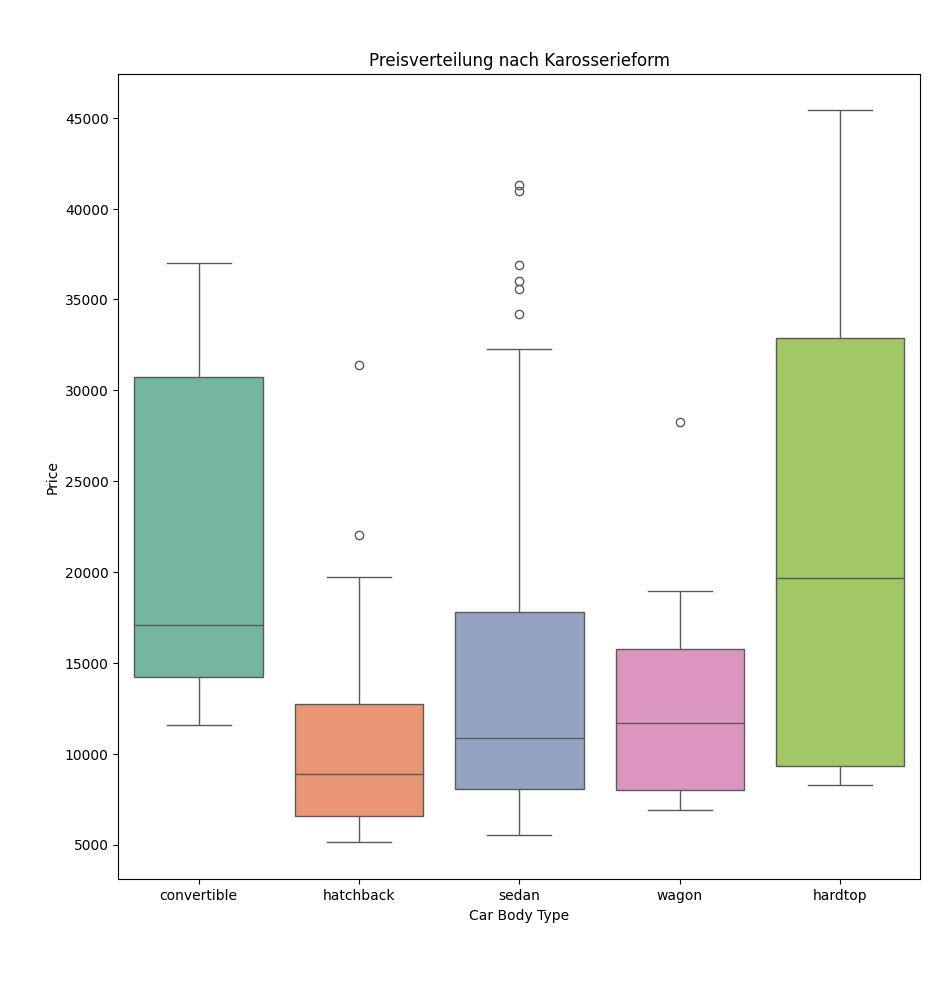
\includegraphics[width=0.8\textwidth]{../images/preisverteilung_nach_karrosserie.png} % Pfad zur Datei anpassen
    \caption{Boxplot der Preisverteilung nach Karosserieform}
    \label{fig:vis1}
\end{figure}

\paragraph{Beschreibung der Visualisierung} \break
Die Abbildung zeigt die Preisverteilung der verschiedenen Karosserieformen als Boxplot.
Aus der Visualisierung lassen sich der Durchschnitsspreis jeder Karosserieform, die Minimal- und Maxiamlwerte, das
obere und untere Quartil sowie gegebenenfalls einzelne Ausreißer ablesen.

\paragraph{Begründung der Wahl}
Für die Darstellung als Boxplot habe ich mich entschieden, da sowohl zentrale Tendenzen (Median), als auch die Streuung der
Preise einschließlich Extrema und Außreiser abgebildet werden. So lassen sich Unterschiede in der Preisverteilung klar erkennen.

\paragraph{Verwendete Datenattribute}
\begin{itemize}
  \item \textbf{price} - Fahrzeugpreis in US-Dollar
  \item \textbf{Car Body Type} - Karosserieform 
\end{itemize}

\hfill \break

\paragraph{Beantwortbare Fragen}
\begin{itemize}
  \item Welche Karosserieform weist den höchsten (\textbf{hardtop}) bzw. den geringsten Durchschnitsspreis auf(\textbf{hatchback})?
  \item Welche Karosserieform hat eine eher geringe Preisspanne (\textbf{hatchback, wagon}), bzw. welche eine sehr große (\textbf{hardtop})?
  \item Welche Karosserieformen zeigen eine große Preisstreuung oder Ausreißer
\end{itemize}

% ===========================
\section{Visualisierung: Beziehung zwischen Leistung und Kraftstoffeffizienz}
\begin{figure}[H]
    \centering
    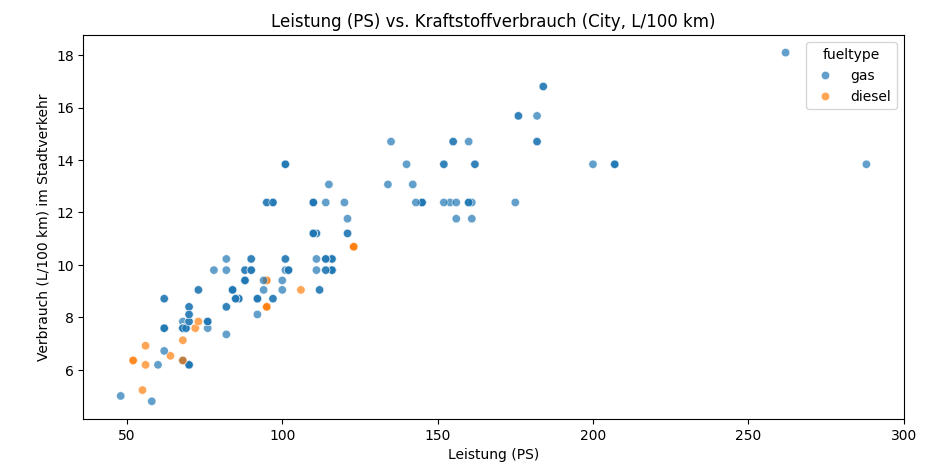
\includegraphics[width=0.8\textwidth]{../images/leistung_vs_kraftstoffeffizienz_lp100.png} % Pfad zur Datei anpassen
    \caption{Scatterplot: Leistung vs. Kraftstoffeffizienz (City MPG)}
    \label{fig:vis2}
\end{figure}

\paragraph{Beschreibung der Visualisierung} \break
Die Abbildung zeigt die Beziehung zwischen der Motorleistung (PS) und der Kraftstoffeffizienz (\textit{Liter pro 100 Kilometer}) als Scatterplot.
Jeder Punkt der Abbildung repräsentiert ein Fahrzeug, die Farbe des jeweiligen Punktes gibt an, ob das Fahrzeug mit Benzin oder Diesel betrieben wird.


\paragraph{Begründung der Wahl}
Mithilfe eines Scatterplots kann die Korrelation zwischen zwei numerischen Variablen, in diesem Fall Motorleistung und Kraftstoffeffizienz,
gut dargestellt werden, da sich Trends, Zusammenhänge und Außreiser unmittelbar visuell erkennen lassen.
Durch die farbliche Unterscheidung der Punkte nach Kraftstofftyp wird zudem sichtbar, ob sich Benzin- und Dieselfahrzeuge hinsichtlich ihres Verbrauchsverhaltens unterscheiden.


\paragraph{Verwendete Datenattribute}
\begin{itemize}
  \item \textbf{horsepower} - Motorleistung (PS)
  \item \textbf{citympg} - Kraftstoffeffizienz (Miles per Gallon im Stadtverkehr)
  \item \textbf{fueltype} - Kraftstoffart (Benzin oder Diesel)
\end{itemize}


\paragraph{Zusätzliche Berechnung} \break
Da in Deutschland der Verbrauch typischerweise \textit{L/100k} angegeben wird, habe ich die Miles Per Gallon im Stadtverkehr in die entsprechenden \textit{L/100k} umgerechnet.
Dafür habe ich folgende Formel verwendet: \break

Grundlage für die Umrechnung sind folgende Werte: \break

\[
1\,\text{mile} = 1.609344\,\text{km}, 
\qquad 
1\,\text{gallon} = 3.785411784\,\text{L}.
\]
Basierend auf diesen Werten ergibt sich:
\[
\begin{aligned}
1\,\text{mpg} 
&= \frac{1\,\text{mile}}{1\,\text{gallon}} \\[6pt]
&= \frac{1.609344\,\text{km}}{3.785411784\,\text{L}} \\[6pt]
&= 0.4251437\,\frac{\text{km}}{\text{L}} \\[10pt]
\Rightarrow \quad
1\,\frac{\text{km}}{\text{L}} 
&= \frac{1}{0.4251437}\,\text{mpg} 
= 2.35215\,\text{mpg} \\[10pt]
\Rightarrow \quad
1\,\text{mpg} 
&= 0.425144\,\frac{\text{km}}{\text{L}} \\[10pt]
\text{Da} \quad
1\,\text{L}/100\,\text{km} 
&= \frac{100}{\text{km}/\text{L}}, \\[6pt]
\text{folgt:} \quad
\text{L/100\,km} 
&= \frac{100}{0.425144 \times \text{mpg}} \\[6pt]
&= \frac{235.215}{\text{mpg}}
\end{aligned}
\]

Die Umrechnung konnte im Python-Skript also mit folgender Formel umsetzen:
\[
\boxed{\text{L/100\,km} = \frac{235.215}{\text{mpg}}}.
\]

\hfill \break


\paragraph{Beantwortbare Fragen}
\begin{itemize}
  \item Gibt es einen Zusammenhang zwischen den PS eines Autos und dem Benzinverbrauch? - 
    \textbf{Ja, es lässt sich ein klarer Zusammenhang zwischen den Werten erkennen}.
  \item Existiert ein Unterschied zwischen dem leistungsabhängigen Verbrauch von Fahrzeugen, die mit Diesel betrieben werden, gegenüber
    Fahrzeugen, die mit Benzin betrieben werden? - \textbf{Nein, es ist kein Unterschied zwischen Diesel- und Benzinfahrzeugen erkennbar}.
\end{itemize}


% ===========================
\section{Visualisierung: Preisstruktur nach Marke und Karosserieform}
\begin{figure}[H]
    \centering
    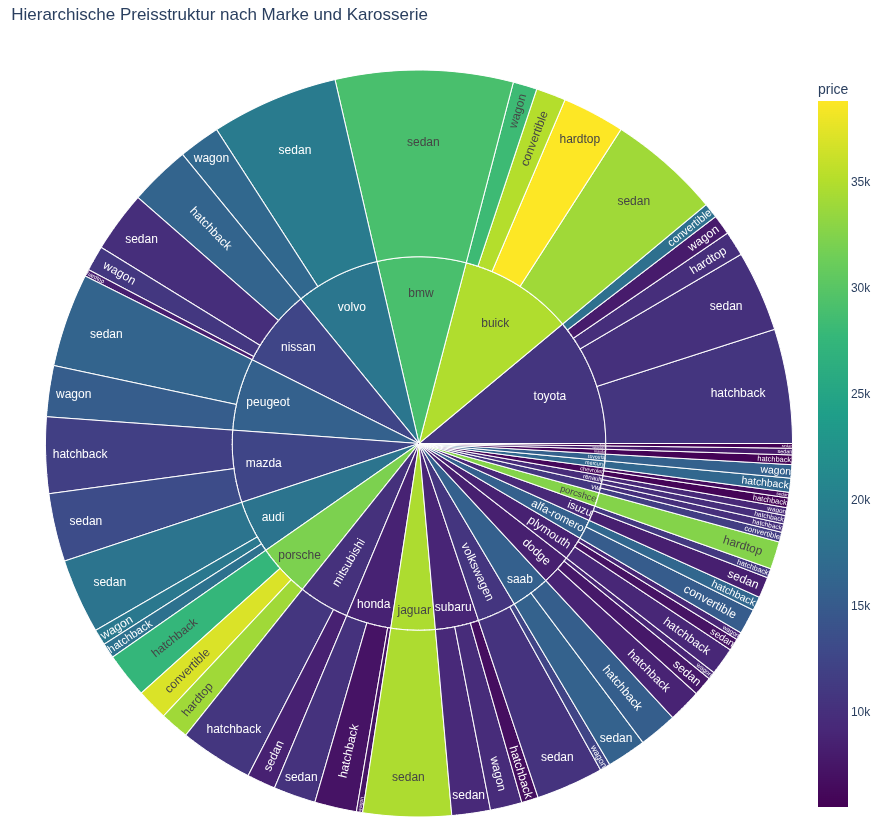
\includegraphics[width=0.8\textwidth]{../images/preisstruktur_nach_marke_karosserie.png} % Pfad zur Datei anpassen
    \caption{Sunburst-Diagramm: Preisstruktur nach Marke und Karosserieform}
    \label{fig:vis3}
\end{figure}


\paragraph{Beschreibung}
Das Sunburst-Diagramm zeigt die hierarchische Preisstruktur der Fahrzeuge nach Marke und Karosserieform.
Jeder Sektion im äußeren Ring repräsentiert eine Karosserieform innerhalb einer Marke, während die Sektionen des inneren Rings die unterschiedlichen Marken repräsentieren.
Durch Interaktivität (in der erstellten Version) kann eine Marke ausgewählt werden, um eine Detailansicht zu erhalten.

\begin{figure}[H]
    \centering
    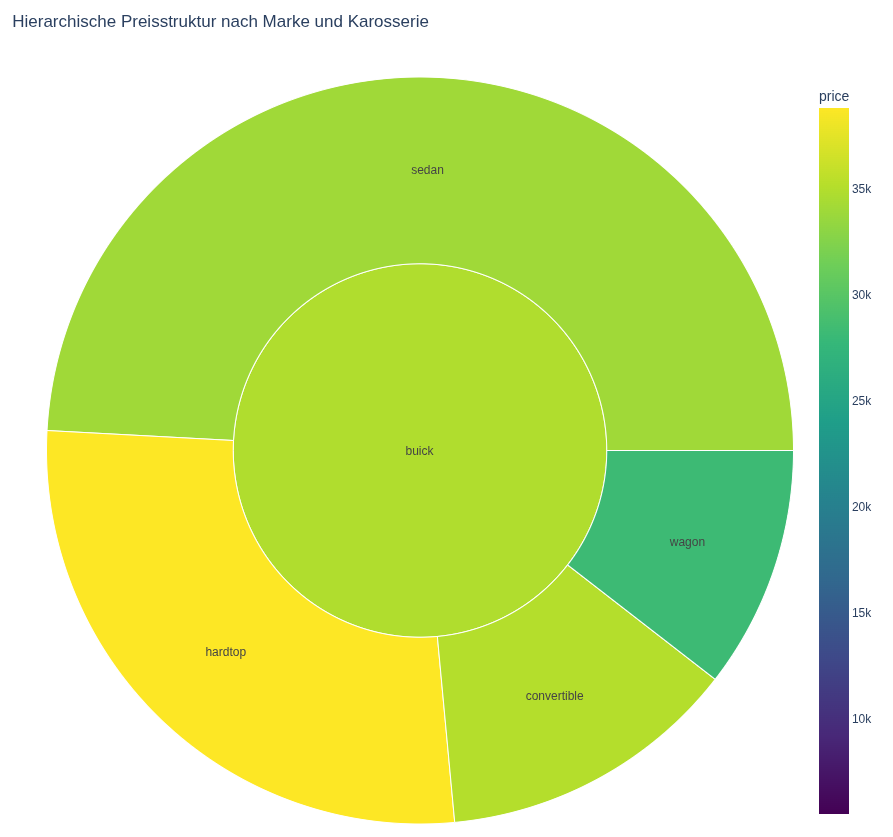
\includegraphics[width=0.8\textwidth]{../images/preisstruktur_nach_marke_karosserie_clicked.png} % Pfad zur Datei anpassen
    \caption{Detailansicht: Preisstruktur der Karosserieformen einer Marke}
    \label{fig:vis4}
  \end{figure}



\hfill \break

\paragraph{Beantwortbare Fragen}
\begin{itemize}
  \item Welche Marken haben einen besonders hohen durchschnittlichen Fahrzeugpreis? - \textbf{buick, jaguar}
  \item Welche Marken haben einen besonders niedrigen durchschnittlichen Fahrzeugpreis? - \textbf{honda, subaru}
  \item Wie unterscheiden sich die Fahrzeugpreise einer Marke abhängig von der Karosserieform?
  \item Welche Karosserieformen haben markenübergreifend durchschnittlich höhere bzw. geringere Durchschnittspreise?
\end{itemize}


% ===========================
\section{Verwendete Tools}
Für die Erstellung der Visualisierungen wurde Python mit folgenden Libraries verwendet:

\begin{itemize}
  \item \textbf{pandas} - Einlesen und Verarbeitung der CSV-Daten
  \item \textbf{matplotlib} - Erstellen statischer Diagramme (Grundlage für Scatterplots und Boxplots) 
  \item \textbf{seaborn} - Erweiterte grafische Darstellung und Stiloptimierung.
    Genutzt für Scatterplots und Boxplots und die Anpassung von Farben und Transparenz.
  \item \textbf{plotly.express} - Erstellung interaktiver Diagramme (Sunburst)
\end{itemize}


\end{document}
